\chapter{Solution development}

\section{Total behaviour}

The behavior of each robot is modeled using a non-deterministic finite state automata (\textit{NFA})(see figure \ref{fig:NFA}). Such an architecture has been chosen for the robot since its behavior is not trivial and more tasks must be executed at different times. By using a FSA, it is easy to explicitly express activities, conditions and non-deterministic transitions. Moreover, each state can be developed separately from the others, and the most suitable solution can be implemented case by case.

\noindent
The robot starts in the ``resting'' state. A non-deterministic transition makes the robot leave the base and start the exploration with a probability $P1$. 

\noindent
When exploring, the robot looks for any close landmark and, if it is the case, it joins the cluster around such landmark with a probability $P2$ and enters in ``waiting for cluster to complete" state. Moreover, the robot may quit the exploration task at any moment and return to the base with a probability $P3$. In the latter casuistry, the robot enters in the ``returning to base" state.

\noindent
When a cluster is completed by reaching the required number of robots $N$, the robot enters in the ``reconnaissance'' state. Such a state conceptually correspond to the phase during which the robots in the cluster should explore the area near the landmark. Such a task is not executed in this project for simplicity, but few different algorithms have been created to let a set of robots to explore and map a given area.

\noindent
The robot ends the reconnaissance task after $t_1$ seconds, and it returns to the base.

\noindent
When returning to the base, the robot executes a phototaxis task. The robot enters in the ``resting'' state once it is detected that it successfully returned to the base. 

\noindent
In the end, the robot may leave the cluster before it is completed with a probability $P4$. In this case, it enters in the ``biased exploration" state, that is a state where the robot executes the regular exploration tasks
but with inhibited stimuli from landmarks. After $t_2$ seconds it returns in the normal exploration behaviour. Such a intermediate state is required so that the robot may step away from the landmark (otherwise, even though it is a probabilistic transition, it would join the cluster again in most of the cases). TODO: required?  

\begin{figure}[H]
\centering
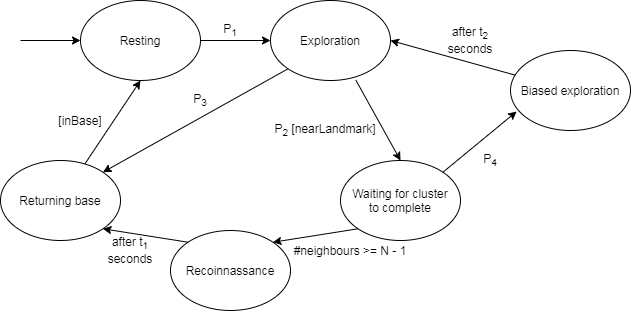
\includegraphics[width=\linewidth]{images/NFA.png}
\caption{\textit{NFA representing the behaviour of the robot. $P_i$ represent a non-deterministic transition that happens with such probability.}}
\label{fig:NFA}
\end{figure}

The implementation of the FSA is executed by using a ``states`` table to store the code be executed in each state. The variable ``current\_state'' represents the current active state, while transition are executed by checking simple``if-then-else'' conditions.

\noindent
In the end, a variable ``t'' stores the time spent by the robot in the current state.

\section{Resting}

The robot in this state just checks if a transition to the exploration one should occur. The following function has been used to model the probability:

\begin{center}
$$ p = tanh((t - Shift) / Patience) + 1 $$
\end{center} 

\noindent
The idea is to create a probability that is directly proportional to the time spent in the current state using a non linear relation. Moreover, the probability should grow very slowly at the beginning so that the robot will remain in the resting state for a while. 

\noindent
The function $tanh(x)$ is the basic function used to represent such relation\footnote{A reasonable alternative would be the exponential function, but it requires the tuning few parameters so that the ``tail'' of the function take reasonable values} (figure \ref{fig:tanh}). The $Shift$ value is constant (500) so we can take the slice of the function having up concavity. The $Patience$ value is a parameter used to tone all values down. In the end, the $+1$ factor let the function have positive values.  

\noindent
Table \ref{tab:f-values} reports few reference values of the function.

\begin{table}[H]
\centering
\begin{tabular}{| c | c |}

\hline
t & p \\
\hline
 0  & 0.013 \\
 10 & 0.015 \\
 50 & 0.022 \\
100 & 0.036 \\
500 & 1 \\
\hline

\end{tabular}
\caption{\label{tab:f-values}\textit{Few example values of the function used to model dependency with elapsed time using a non linear relation.}}
\end{table}

\begin{figure}[H]
\centering
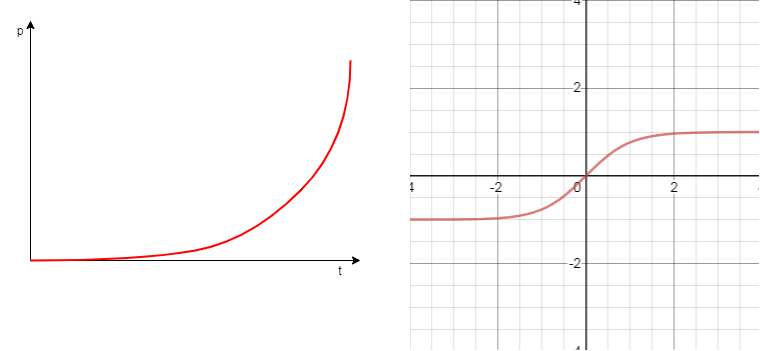
\includegraphics[width=\linewidth]{images/tanh.png}
\caption{\textit{A template of the expected function (left) and the regular tanh function (right).}}
\label{fig:tanh}
\end{figure}

\section{Exploration}

\section{Clustering}

\section{Returning to base}
